\chapter{脉冲星计时阵列对原初黑洞丰度的限制}\label{chap:PTAfPBH}

%The detection of binary black hole coalescences by LIGO/Virgo has aroused the interest in primordial black holes (原初黑洞), because they could be both the progenitors of these black holes and a compelling candidate of dark matter (暗物质). 原初黑洞 are formed soon after the enhanced scalar perturbations re-enter horizon during radiation dominated era, which would inevitably induce  gravitational waves as well. Searching for such scalar induced gravitational waves (标量诱导引力波) provides an elegant way to probe 原初黑洞. We perform the first direct search for the signals of 标量诱导引力波 accompanying the formation of 原初黑洞 in North American Nanohertz Observatory for Gravitational waves (NANOGrav) 11-year data set. No statistically significant detection has been made, and hence we place a stringent upper limit on the abundance of 原初黑洞 at $95\%$ confidence level. In particular, less than one part in a million of the total 暗物质 mass could come from 原初黑洞 in the mass range of $[2 \times 10^{-3}, 7\times 10^{-1}] \Msun$.

\section{研究背景}
在过去的几年里,\lvc 科学组织不仅探测到来自双黑洞并合\cite{Abbott:2016blz,Abbott:2016nmj,Abbott:2017vtc,  Abbott:2017gyy,Abbott:2017oio,TheLIGOScientific:2016pea,LIGOScientific:2018mvr}产生的引力波,而且探测到了双中子星并合\cite{TheLIGOScientific:2017qsa}产生的引力波。\lvc 取得的重大科学成就使得人类进入了引力波天文学和多信使天文学的新时代。为了解释\lvc 探测到的双黑洞是如何形成和演化的,人们提出了众多模型\cite{Fishbach:2017dwv,Antonini:2016gqe,Inayoshi:2017mrs,Perna:2019axr,Rodriguez:2015oxa,Rodriguez:2016kxx,Park:2017zgj,Belczynski:2014iua,Belczynski:2016obo,Woosley:2016nnw,Rodriguez:2018rmd,Choksi:2018jnq,deMink:2010zm,deMink:2016vkw,Bird:2016dcv,Sasaki:2016jop,Clesse:2016vqa,Wang:2016ana,Ali-Haimoud:2017rtz,Chen:2018czv,Chen:2018rzo,Kavanagh:2018ggo,Raidal:2018bbj,Liu:2018ess,Chen:2019irf,Yuan:2019udt,Liu:2019rnx}。作为其中的一种模型,原初黑洞模型\cite{Bird:2016dcv,Sasaki:2016jop,Chen:2018czv}最近引起了很多关注。在宇宙早期,原初黑洞是在标量曲率扰动的波长重新进入视界的时候,由于过密区域发生引力坍缩而产生的\cite{Ivanov:1994pa,Yokoyama:1995ex,GarciaBellido:1996qt,Ivanov:1997ia,Kawasaki:2006zv}。在这种情况下,原初黑洞的质量与视界质量相当\cite{Carr:1975qj},从而导致原初黑洞的质量谱比天体物理学黑洞的质量谱宽得多。

原初黑洞模型之所以吸引人,是因为它不仅可以解释\lvc 探测到的双黑洞并合事件的事件率,而且也是暗物质的候选者之一。暗物质问题仍然是困扰人类的一个未解之谜。
原初黑洞能否构成所有的暗物质还没有定论。然而原初黑洞占冷暗物质的丰度$\fpbh$
已经受到各种实验观测,例如原初黑洞产生的银河系外$\gamma$射线 \cite{Carr:2009jm}、$\gamma$射线暴的femtolensing\cite{Barnacka:2012bm}、Subaru/HSC微透镜\cite{Niikura:2017zjd}、开普勒毫/微透镜\cite{Griest:2013esa}、OGLE微透镜\cite{Niikura:2019kqi}、EROS/MACHO微透镜\cite{Tisserand:2006zx}、
本星系中的白矮星\cite{Graham:2015apa}、超暗矮星系的动态加热\cite{Brandt:2016aco}、
原初黑洞吸积星际气体产生的X射线/无线电辐射\cite{Gaggero:2016dpq}、原初黑洞吸积原初气体产生的宇宙微波背景辐射\cite{Ali-Haimoud:2016mbv,Blum:2016cjs,Horowitz:2016lib,Chen:2016pud}、亚太阳质量双黑洞并合产生的引力波\cite{Abbott:2018oah,Magee:2018opb,Chen:2019irf,Authors:2019qbw}和双黑洞并合产生的随机引力波背景\cite{Wang:2016ana,Chen:2019irf}。但是在$[10^{-16},10^{-14}] \cup [10^{-13},10^{-12}] M_\odot$的质量窗口内,原初黑洞仍然可能构成所有的暗物质。请参考文献\cite{Chen:2019irf}里关于原初黑洞实验限制的最新总结。

我们知道,在原初黑洞形成的过程中,由于曲率标量扰动将不可避免地产生标量诱导引力波。所以通过标量诱导引力波也可以探测原初黑洞暗物质。最近,研究表明标量诱导引力波背景的能量密度谱和其他引力波源的能量密度谱具有显著区别\cite{Yuan:2019wwo}。由于原初黑洞应该是由曲率扰动概率密度的尾部形成的,所以形成单个原初黑洞的概率对曲率扰动功率谱的振幅相当敏感\cite{Young:2014ana}。因此,原初黑洞的丰度对相应标量诱导引力波的振幅极为敏感。因此如果探测到标量诱导引力波的将为原初黑洞的存在提供证据;而如果没有探测到标量诱导引力波将对原初黑洞的丰度产生严格的限制。


标量诱导引力波的峰值频率$(f_*)$由共动曲率扰动的功率谱的峰值,因此与原初黑洞的质量有如下关系\cite{Saito:2008jc}
\e
f_*\sim 3\,{\rm{Hz}}\({m_{\rm{PBH}}/10^{-18} M_\odot}\)^{-1/2}.
\q
构成暗物质的原初黑洞的质量应重于$10^{-18}\Msun$,否则它们会因霍金辐射而蒸发。相应的标量诱导引力波的峰值频率应该低于$3$Hz,因此地基引力波探测器很难探测到相应的标量诱导引力波。另一方面,低频引力波探测器特别适合探测原初黑洞暗物质。文献\cite{Yuan:2019udt}预测了LISA\cite{Audley:2017drz}以及脉冲星计时阵列(如IPTA\cite{Hobbs:2009yy}、FAST\cite{Nan:2011um}和SKA\cite{Kramer:2015jsa})对原初黑洞丰度所能达到的观测限制。相关的工作请参见\cite{Inomata:2016rbd,Schutz:2016khr,Orlofsky:2016vbd,Dror:2019twh,Wang:2019kaf,Cai:2019elf,Clesse:2018ogk}。

尽管目前脉冲星计时阵列的数据已经被用来限制随机引力波背景的振幅,但这些结果强烈地依赖于一些特殊的幂律形式的假设,而这种幂律形式与标量诱导引力波完全不同\cite{Yuan:2019udt}。在本节中,我们将首次在公开的脉冲星计时阵列的数据集中搜索标量诱导引力波的信号,以检验原初黑洞暗物质假设。我们在NANOGrav 11年数据集中未探测到标量诱导引力波,进而给出了质量范围为$[4\times 10^{-4}, 1.7]\Msun$的原初黑洞丰度的限制。

%%%%%%%%%%%%%%%%%%%%%%%%%%%%%%%%%%%%%%%%%%%%%%%%%%%%%%%%%%%%%%%%%%%%%%%%%%%%%%%%

\section{原初黑洞的形成机制}

在这里,我们只考虑了原初黑洞具有单色质量谱的情况,其对应于$\delta$功率谱的标量曲率扰动,即
\e\label{pzeta1}
\mathcal{P}_{\zeta}(k)=A k_*\delta\(k-k_*\),
\q
其中$A$是功率谱的无量纲振幅。在这种情况下,原初黑洞的质量与峰值频率$f_*$的关系为\cite{Hawking:1971ei,Carr:1974nx}
\m\label{mkrelation}
{m_{\mathrm{PBH}}\over M_{\odot}} \simeq 2.3\times10^{18}%\left(\frac{3.91}{g_*^{\mathrm{form}}}\right)^{1 / 6}
\left(\frac{H_{0}}{f_*}\right)^{2},
\n
其中$f_*$的单位是Hz,$H_0$是哈勃常数。原初黑洞的形成是一个阈值过程,它是由高斯随机场(Gaussian random fields)的三维统计描述的,也称为峰值理论(peak theory)\cite{Bardeen:1985tr}。

在宇宙早期,由于宇宙的能量密度对原初黑洞的形成起关键作用\cite{Hawking:1971ei, Carr:1974nx},所以在形成时,原初黑洞的质量$M$和视界质量大致有如下关系
\begin{align}
    M
    &\sim
    \frac{ t }{ G }
    \sim
    10^{15}\,
    \left(
    \frac{t}{10^{-23}\,\srm}
    \right)\,
    \grm
    \, .
    \label{eq:Moft}
\end{align}
因此,原初黑洞的质量可以横跨很多个数量级。例如,在普朗克时间($10^{-43}\,\srm$)形成的原初黑洞的质量为普朗克质量($10^{-5}\,\grm$),而在$1\,\srm$形成的原初黑洞的质量可以达到$10^{5}\, M_{\odot}$。早期宇宙的高能量密度是形成原初黑洞的必要条件,但不是充分条件。如果早期宇宙存在原初不均匀性,那么高密度区域可能会停止膨胀并塌缩形成原初黑洞。在这种情况下,\Eq{eq:Moft}可以被更精确地表达为\cite{Carr:2009jm}
\begin{equation}
    M
    \approx
    2.03 \times 10^{5}\,
    \gamma
    \left( \frac{t}{1\,\srm} \right)
    M_{\odot}
    \, .
    \label{mass}
\end{equation}
其中$\gamma$是一个取决于塌缩过程的系数。在辐射为主时期,$\gamma = (1 / \sqrt{3\,})^{3} \approx 0.4$ \cite{Green:2004wb}。

我们用$\beta( M )$表示质量为$M$的原初黑洞在形成时占宇宙质量的百分数,则有\cite{Carr:2009jm}
\begin{equation}
    \beta( M )
    \equiv
    \frac{M\,n_{\mathrm{PBH}}(t_{\irm})}{\rho(t_{\irm})}
    \approx
    7.98 \times 10^{-29}\,
    \gamma^{-1/2}\,
    \left( \frac{M}{M_{\odot}} \right)^{\!3/2}\,
    \left( \frac{n_{\mathrm{PBH}}(t_{0})}{1\,\mathrm{Gpc}^{-3}} \right)
    ,
    \label{eq:beta}
\end{equation}
其中$t_{\irm}$为原初黑洞的形成时间,$n_{\mathrm{PBH}}$为原初黑洞的数密度,$g_{* \irm}$为原初黑洞形成时的相对论自由度。在今天为蒸发的原初黑洞的能量密度参数$\Omega_{\mathrm{PBH}}$大致为\cite{Carr:1975qj}
\begin{equation}
    \Omega_{\mathrm{PBH}}
    =
    \frac{M\,n_{\mathrm{PBH}}( t_{0} )}{\rho_{\mathrm{crit}}}
    \approx
    \left( \frac{\beta( M )}{1.03 \times 10^{-8}} \right)
    \left( \frac{h}{0.68} \right)^{\!-2}
    \gamma^{1/2}\,
    \left( \frac{g_{* \irm}}{106.75} \right)^{\!-1/4}\,
    \left( \frac{M}{M_{\odot}} \right)^{\!-1/2}
    \,.
    \label{eq:omega}
\end{equation}
通过峰值理论可以算出原初黑洞数密度,从而求出原初黑洞在暗物质中的丰度\cite{Carr:2016drx}
\m\label{fpbh}
f_{\mathrm{PBH}}\equiv\Omega_{\mathrm{PBH}}/\Omega_{\mathrm{DM}} \simeq 1.9 \times 10^{7}
\({\zeta_c^2/A}-1\) e^{-{\zeta_c^2\over 2A}} \left(\frac{m_{\mathrm{PBH}}}{M_{\odot}}\right)^{-\frac{1}{2}},
\n
其中$\zeta_{c}\simeq1$ \cite{Musco:2008hv,Musco:2004ak,Musco:2012au,Harada:2013epa,Escriva:2019nsa,Escriva:2019phb}是形成原初黑洞的阈值。

\section{标量诱导引力波}
标量诱导引力波可以用扰动理论来计算。以往的文献只考虑标量诱导引力波的二阶修正。在这里,我们考虑诱导引力波到三阶修正。为此,我们需要将爱因斯坦方程展开到到四阶。扰动的的FRW度规为
\e
\rd s^{2}=a^{2}\left\{-(1+2 \phi) \rd \eta^{2}+\left[(1-2 \phi) \delta_{i j}+\frac{h_{i j}}{2}\right] \rd x^{i} \rd x^{j}\right\},
\q
其中$\phi$为标量扰动,$h_{ij}$为张量扰动。傅立叶空间的标量扰动具有如下形式的解\cite{Baumann:2007zm,Kohri:2018awv,Sasaki:2018dmp}
\e\label{phi}
\phi_{\vec{k}}(\eta) \equiv \phi_{\vec{k}}T(k\eta),
\q
其中$\phi_{\vec{k}}$为原初扰动,且$T(k\eta)$为转移函数
\e\label{transfer}
T(k\eta) =  \frac{9}{(k\eta)^2} \[ \frac{\sin(k\eta/\sqrt{3})}{k\eta/\sqrt{3}} - \cos(k\eta/\sqrt{3})\].
\q
在辐射主导时期,转移函数随时间振荡衰减,即$T(k\eta)\sim1/\eta^2$。我们用\texttt{xPand} \cite{Pitrou:2013hga}软件包来将爱因斯坦方程展开到四阶。经过繁杂的计算,我们得到如下的运动方程
\e\label{eqh}
h_{i j}^{\prime \prime}+2 \mathcal{H} h_{i j}^{\prime}-\nabla^{2} h_{i j}=-4 \mathcal{T}_{i j}^{\ell m} S_{\ell m},
\q
其中一撇代表对共形时间$\eta$的导数,$\mH \equiv a'/a$为共形哈勃参数,且$\mathcal{T}_{i j}^{\ell m}$为TT投影算符\cite{Ando:2017veq}。尽管\Eq{eqh}和二阶的引力波扰动方程具有相同的形式(例如见\cite{Ando:2017veq,Baumann:2007zm}),然而源项却不一样。我们将源项$S_{ij}=\Sij{2}+\Sij{3}+\Sij{4}$计算到四阶,具体为
\e\label{S2}
\Sij{2}= 4 \phi \p_i\p_j\phi + 2\p_i\phi\p_j\phi-\p_i \(\phi + {\phi'\over\mH}\)
\p_j\(\phi + {\phi'\over\mH}\),
\q
%\m
%\Sij{2} = 4 \phi \phi_{ij} + 2\phi_i\phi_j-\frac{1}{\mH} \(\phi_i + { \phi_i'\over\mH}\)
%\(\phi_j + {\phi_j'\over\mH}\),
%\n	
\e\label{S3}
\begin{split}
    \Sij{3} =& \frac{1}{\mH} \(12\mH \phi - \phi'\) \p_i\phi \p_j\phi
    - \frac{1}{\mH^3} \(4\mH \phi - \phi'\)\p_i\phi'\p_j\phi' \\
    &+ \frac{1}{3\mH^4} \(2\p^2\phi - 9\mH \phi'\) \p_i\(\mH\phi +\phi'\)
    \p_j\(\mH\phi +\phi'\),
\end{split}
\q
%\m
%\Sij{3} &&= \frac{1}{\mH} \(12\mH \phi - \phi'\) \phi_i \phi_j
%- \frac{1}{\mH^3} \(4\mH \phi - \phi'\)\phi_i'\phi_j'\no\\
%&&+ \frac{1}{3\mH^4} \(2\p^2\phi - 9\mH \phi'\) \(\mH \phi_i + \phi_i'\)
%\(\mH\phi_j + \phi_j'\),
%\n
\e\label{S4}
\begin{split}
    \Sij{4} =& 16 \phi^3 \p_i\p_j\phi
    + \frac{1}{3\mH^3} \Big[2 \phi' \p^2\phi - 9\mH \phi'^2 
    - 8\mH \phi \p^2\phi + 18 \mH^2 \phi \phi'
    + 96\mH^3 \phi^2\Big] \p_i\phi\p_j\phi \\
    &+ \frac{2}{3\mH^5} \Big[- \phi' \p^2\phi + 3\mH \phi'^2 
    + 4\mH \phi \p^2\phi + 3 \mH^2 \phi \phi'- 12\mH^3 \phi^2\Big] \p_i\phi' \p_j\phi'\\
    &+ \frac{1}{36\mH^6} \Big[ 
    -16 (\p^2\phi)^2 - 3  \partial_k\phi' \partial^k\phi'
    + 120 \mH \phi' \p^2\phi - 6 \mH \partial_k\phi \partial^k\phi'	\\
    &\qquad\qquad + 144 \mH^2 \phi \p^2\phi - 180 \mH^2 \phi'^2 
    + 33 \mH^2 \partial_k\phi \partial^k\phi- 504 \mH^3 \phi \phi'
    - 144 \mH^4 \phi^2
    \Big] \\
    &\qquad\qquad\times  \p_i\(\mH\phi +\phi'\)
    \p_j\(\mH\phi +\phi'\).
\end{split}
\q

在傅立叶空间用格林函数法解\eqref{eqh}可得到\cite{Baumann:2007zm}
\e\label{hsol} 
h(\vec{k},\eta) = \frac{1}{k a(\eta)} \int \rd \te \sin(k\eta - k\te) a (\te) \mathcal{S}_{\vec{k}}(\te),
\q 
其中$\mathcal{S}_{\vec{k}}(\eta)\equiv -4e^{ij}(\vec{k}) \tilde{S}_{ij}(\vec{k},\eta)$,而$\tilde{S}_{ij}(\vec{k},\eta)$为源项在傅立叶空间的表达式。$+$和$\times$模式的引力波极化张量$e_{ij}(\vec{k})$分别为$(e_i e_j - \bar{e}_i \bar{e}_j)/\sqrt{2}$和$(e_i \bar{e}_j + \bar{e}_i e_j)/\sqrt{2}$,其中$e_i(\vk)$ 和$\bar{e}_i(\vk)$为两个垂直于传播方向$\vk$的相互独立的单位矢量。在超视界尺度,由于标量扰动$\phi$和共动曲率扰动$\zeta$的关系为$\phi = (2/3) \zeta$,所以引力波的能量密度参数$\ogw(\eta, k)$可以通过共动曲率扰动的功率谱 $\mathcal{P}_{\zeta}(k)$来计算。$\mathcal{P}_{\zeta}(k)$的定义为
\e
\left\langle \zeta_{\vk} \zeta_{\vec{k'}}\right\rangle\equiv\frac{2 \pi^{2}}{k^{3}} \mathcal{P}_{\zeta}(k) \delta(\vec{k}+\vec{k'}). 
\q

对于\Eq{pzeta1}的$\delta$谱,傅立叶空间的源项为
\m
\mathcal{S}^{(2)}_{\vec{k}}(\eta)&\equiv&\int \frac{\rd^3p}{(2\pi)^{3/2}} \be(\bp, \bp)
f_2(\kstar \eta) \zeta_{\bp} \zeta_{\bm{k-p}},\\
\mathcal{S}^{(3)}_{\vec{k}}(\eta)&\equiv&\int \frac{\rd^3p \rd^3q}{(2\pi)^3} \be(\bp, \bq)
f_3(\kstar \eta) \zeta_{\bp} \zeta_{\bq} \zeta_{\bm{k-p-q}},\\
\mathcal{S}^{(4)}_{\vec{k}}(\eta)&\equiv&\int \frac{\rd^3p \rd^3q \rd^3l}{(2\pi)^{9/2}}\[ 
\be(\bl, \bl)+ \be(\bp,\bq)\] f_4(\kstar \eta) \zeta_{\bp} \zeta_{\bq} \zeta_{\bl} \zeta_{\bm{k-p-q-l}},
\n
其中$\be(\bp, \bq) \equiv e^{ij}(\vec{k})p_iq_j$,且$f_i(x)$($i = 2, 3, 4$)具有如下的函数形式 
\m
f_2(x)&=&{8\over9}\(3T^2 + 2xTT' + x^2T'^2\),\\
f_3(x)&=& -\frac{64}{81} \Big[ \(x^2-18\) T^3 + 2x \(3+x^2\) T^2 T' + x^2 \(15 + x^2\) T T'^2 + 3 x^3 T'^3 \Big], \\
f_4(x)&=& {16\over729}\Big[\(720-29x^2+16x^4\)T^4 +x^4 \(108 + 7 x^2\) T'^4 +4x^3\(198 + 31 x^2\)TT'^3\no\\
&& +2x^2\(864+219x^2+8x^4\)T^2T'^2+4x\(144+73x^2+8x^4\)T^3T'\Big].
\n
转移函数$T=T(x)$的表达式由\Eq{transfer}给出。
从\Eq{Ph}和\Eq{hsol}可以看出只有$\av{\mathcal{S}^{(2)}_{\vec{k}} \mathcal{S}^{(2)}_{\vec{k'}}}$对二阶诱导引力波有贡献。同时,$\av{\mathcal{S}^{(3)}_{\vec{k}} \mathcal{S}^{(3)}_{\vec{k'}}}$和$\av{\mathcal{S}^{(2)}_{\vec{k}} \mathcal{S}^{(4)}_{\vec{k'}}}$都对三阶修正有贡献。参照\cite{Espinosa:2018eve,Kohri:2018awv},对于\Eq{pzeta1}的$\dt$谱有
\e\label{ogw}
\ogw(\eta, k)=\frac{A^2}{384\tk^{2}}\Big[\overline{I_2^2}M_1+
A \(M_2\overline{I_3^2}+M_1\overline{I_2 I_4}\)\Big],
\q
其中$I_i$ ($i = 2, 3, 4$)定义为
\e\label{Ii}
I_i = \lim_{x \to \infty} \int_0^x \rd\tx\, f_i\!\!\(\frac{\tx}{\tk}\) 
{\tx\over x} \sin(x-\tx).
\q
为了方便,在上式中我们定义了一些新的变量,即$\tk\equiv k/\kstar$,$x\equiv k\eta$以及 $\tx\equiv k\tilde{\eta}$。和\cite{Kohri:2018awv}类似,\Eq{Ii}可以通过多次利用三角函数的性质化简而得到解析的表达式。\Eq{ogw}中的角度积分$M_1$和$M_2$分别定义为
\m
M_1(k) &=& \(4 - \tk^2\)^2 \Theta(2 - \tk),\\
M_2(k) &=& \frac{1}{\pi^2} \int_{p_{\rm{min}}}^{p_{\rm{max}}} \rd\tp
\int_{0}^{2\pi} \rd\ap \int_{0}^{2\pi} \rd\phi M_0 \Theta(\Delta),
\n
其中$p_{\rm{min}} = |1-\tk|$,且$p_{\rm{max}} = \min(2,1+\tk)$。$M_2$可以通过数值积分而得到。$M_0$和$\Delta$的定义为
\m
\Delta &=& 4\mu^2+4(1-\mu^2)\cos(\al-\phi)^2-\tilde{p}^2,\\
M_0 &=& \sum_{i=1}^{2} \frac{(1-\nu_i^2)}{\left|\mu \sqrt{1-\nu_i^2} 
    - \nu_i \sqrt{1-\mu^2} \cos(\ap-\phi)\right|}\no\\
&&\times \Big[ 
(1-\nu_i^2)^{3\over2} \cos^22\al + 2\tp^3 (1-\mu^2)^{3\over2} \cos2\phi \cos(\al+\phi)\no\\
&&- 2 \tp (1-\nu_i^2) (1-\mu^2)^{\half} \cos2\al\cos(\al+\phi) - \tp^2 (1-\mu^2) (1-\nu_i^2)^{\half} \cos(\al+\phi)^2 \Big],
\n
其中$\mu$和$\nu_i$($i=1,2$)定义为
\m
\mu &=& {\tp^2+\tk^2-1 \over 2\tp \tk}, \\
\nu_{1,2} &=& \frac{\tp\mu\pm\sqrt{1-\mu^2}|\cos(\al-\phi)|\sqrt{\Delta}}{2\((1-\mu^2)\cos(\al-\phi)^2+\mu^2\)}.
\n
需要注意的是$M_1$来自于$\av{\mathcal{S}^{(2)}_{\vec{k}} \mathcal{S}^{(2)}_{\vec{k'}}}$和$\av{\mathcal{S}^{(2)}_{\vec{k}} \mathcal{S}^{(4)}_{\vec{k'}}}$,并对应于截断频率 $k=2\kstar$;而$M_2$来自于$\av{\mathcal{S}^{(3)}_{\vec{k}} \mathcal{S}^{(3)}_{\vec{k'}}}$,并对应于截断频率$k=3\kstar$。所以三阶修正不仅增强了引力波的能力密度,而且将截断频率从$2\kstar$延展到$3\kstar$。

需要注意的是\Eq{ogw}只有在重进入视界到物质辐射平衡时期有效。由于引力波的能力密度和辐射的衰减是一样的,所以今天的能量密度参数可以近似表达为\cite{Espinosa:2017sgp}
\e
\ogw(\eta_0, f) \simeq \Omega_{r} \times \ogw(\eta, f),
\q
其中$\Omega_{r}$为今天的辐射密度参数。

%%%%%%%%%%%%%%%%%%%%%%%%%%%%%%%%%%%%%%%%%%%%%%%%%%%%%%%%%%%%%%%%%%%%%%%%%%%%%%%%

\section{脉冲星计时阵列数据分析}
由于未探测到随机引力波背景,NANOGrav\footnote{\url{http://nanograv.org}}、PPTA\footnote{\url{https://www.atnf.csiro.au/research/pulsar/ppta}}和EPTA\footnote{\url{http://www.epta.eu.org}}等脉冲星计时阵列合作组织给出了随机引力波背景的振幅的上限。例如,NANOGrav不仅限制了超大质量黑洞产生的随机引力波背景,而且限制了其他引力波背景谱(如幂律谱、折幂律谱、自由谱和高斯过程谱\cite{Arzoumanian:2018saf})。PPTA合作组\cite{Shannon:2013wma}和EPTA合作组\cite{vanHaasteren:2011ni}也给出了类似的限制。然而,标量诱导引力波的信号和脉冲星计时阵列组织搜索的引力波信号大不相同。因此,有必要研究标量诱导引力波,从而通过当前的观测数据为原初黑洞暗物质的丰度设定一个上限。在本章中,我们将从NANOGrav 11年数据集中搜索标量诱导引力波的信号。该数据集包含到达时间(time of arrival,TOA)数据和脉冲星计时模型(timing models)\cite{Arzoumanian:2017puf}。与 \cite{Kato:2019bqz}类似,我们选择了6颗TOA精度相对较好、观测时间较长的脉冲星。\Table{pulsars}列出了这些脉冲星的基本性质。对于这6颗脉冲星,$T_{\rm{obs}}$长于$8$年,$N_{\rm{TOA}}$大于$10^4$,RMS小于$1.5\mu s$。
\begin{table}[htb]
    \begin{center}
    \begin{tabular}{ccccc}
        \hline\hline
        脉冲星名称\hspace{1mm} & RMS [$\mu$s]\hspace{1mm} & $N_{\rm{epoch}}$\hspace{1mm} & $N_{\rm{TOA}}$\hspace{1mm} & $T_{\rm{obs}}$ [yr] \\
        \hline    
        J0613$-$0200 & 0.422 & 324 & 11,566 & 10.8  \\
        J1012$+$5307 & 1.07 & 493 & 16,782 & 11.4  \\
        J1600$-$3053 & 0.23 & 275 & 12,433 & 8.1  \\
        J1713$+$0747 & 0.108 & 789 & 27,571 & 10.9  \\
        J1744$-$1134 & 0.842 & 322 & 11,550 & 11.4  \\
        J1909$-$3744 & 0.148 & 451 & 17,373 & 11.2  \\    
        \hline \hline
    \end{tabular}
\bicaption[数据分析中所使用的6颗脉冲星的基本属性:RMS--加权均方根计时残差,$N_{\rm{epoch}}$--观测数,$N_{\rm{TOA}}$--TOA数,$T_{\rm{obs}}$--观测时间跨度。]{数据分析中所使用的6颗脉冲星的基本属性:RMS--加权均方根计时残差,$N_{\rm{epoch}}$--观测数,$N_{\rm{TOA}}$--TOA数,$T_{\rm{obs}}$--观测时间跨度。详见文献\cite{Arzoumanian:2017puf}。}{Basic properties of the $6$ pulsars used in 
our analysis: RMS - the weighted root-mean-square epoch-averaged post-fit timing residuals,
$N_{\rm{epoch}}$ - number of observational epochs,
$N_{\rm{TOA}}$ - number of TOAs,
$T_{\rm{obs}}$ - observational time span.
See Ref.~\cite{Arzoumanian:2017puf} in detail.}     
\label{pulsars}
    \end{center}
\end{table}


%%%%%%%%%%%%%%%%%%%%%%%%%%%%%%%%%%%%%%%%%%%%%%%%%%%%%%%%%%%%%%%%%%%%%%%%%%%%%%%%
\begin{table}[htb!]
    %\begin{center}
    {
    \scriptsize
    \begin{tabular}{llll}
        \hline\hline
        参数 & 描述 & 先验分布 & 注解 \\
        \hline
        %\vspace{0.5em}
        \multicolumn{4}{c}{标量诱导引力波信号} \\[1pt]
        $A$ & 引力波背景的应变振幅 & U$[10^{-5}, 10^{0}]$ (求上限) & \\
        & & logU $[-5, 0]$ (模型比较) & 整个PTA一个参数 \\
        $\fstar$ & 峰值频率 & $\delta$函数  &  \\
        \hline
        % \vspace{0.5em}
        \multicolumn{4}{c}{白噪音} \\[1pt]
        $E_{k}$ & EFAC 白噪音参数 & U$[0, 10]$ & 固定成单颗脉冲星拟合的最佳值 \\
        $Q_{k}$[s] & EQUAD 白噪音参数 & logU$[-8.5, -5]$ & 固定成单颗脉冲星拟合的最佳值 \\
        $J_{k}$[s] & ECORR 白噪音参数 & logU$[-8.5, -5]$ & 固定成单颗脉冲星拟合的最佳值 \\
        \hline
        % \vspace{0.5em}
        \multicolumn{4}{c}{红噪音} \\[1pt]
        $\ARN$ & 红噪音幂率振幅 & U$[10^{-20}, 10^{-11}]$ (求上限) & \\
        & & logU$[-20, -11]$ (模型比较)  & 每颗脉冲星一个参数 \\
        $\gRN$ & 红噪音幂率谱指数 & U$[0, 9]$ & 每颗脉冲星一个参数 \\
        \hline
        % \vspace{0.5em}
        \multicolumn{4}{c}{\textsc{BayesEphem}星历表模型} \\[1pt]
        $z_{\rm drift}$ [rad/yr] & 地球轨道关于黄道面$z$轴的漂移率 & U[$-10^{-9}, 10^{-9}$] & 整个PTA一个参数 \\
        $\Delta M_{\rm jupiter}$ [$M_{\odot}$] & 木星质量的微扰 & $\mathcal{N}(0, 1.55\times 10^{-11})$  & 整个PTA一个参数 \\
        $\Delta M_{\rm saturn}$ [$M_{\odot}$] & 土星质量的微扰 & $\mathcal{N}(0, 8.17\times 10^{-12})$  & 整个PTA一个参数 \\
        $\Delta M_{\rm uranus}$ [$M_{\odot}$] & 天王星质量的微扰 & $\mathcal{N}(0, 5.72\times 10^{-11})$  & 整个PTA一个参数 \\
        $\Delta M_{\rm neptune}$ [$M_{\odot}$] & 海王星质量的微扰 & $\mathcal{N}(0, 7.96\times 10^{-11})$  & 整个PTA一个参数 \\
        PCA$_{i}$ & 木星轨道分量的微扰 & U$[-0.05, 0.05]$ & 整个PTA六个参数 \\
        \hline
    \end{tabular}
\bicaption{在NANOGrav 11年数据中搜索标量诱导引力波所使用的参数及其先验分布。我们用U表示平的分布,logU表示对数平的分布,及$\mathcal{N}$表示高斯分布。}{Parameters and their prior distributions used in the searching for scalar induced gravitational waves in NANOGrav 11-yr data set. We use U, logU and $\mathcal{N}$ to denote uniform, log uniform and Gaussian distributions, respectively.}
\label{tab:priors}
}
    %\end{center}
\end{table}
%%%%%%%%%%%%%%%%%%%%%%%%%%%%%%%%%%%%%%%%%%%%%%%%%%%%%%%%%%%%%%%%%%%%%%%%%%%%%%%%

随机引力背景的存在将表现为脉冲星信号的到达时间中扣除各种噪音后的残差。这一残差是在考虑了脉冲星自旋行为导致的计时模型及脉冲星与地球运动所产生的几何效应之后仍存在的残差 \cite{1978SvA....22...36S,Detweiler:1979wn}。因此,通过定期监测来自那些自旋稳定的毫秒脉冲星的到达时间,有可能将引力波诱导的残差(这些残差在不同的脉冲星之间有明显的相关性)与其他系统效应(如时钟误差或光在星际介质中传播造成的延迟)分离开来\cite{1990ApJ...361..300F}。对于单个脉冲星,用$\dt \bm{t}$代表长度为$\NTOA$的定时残差向量,则有 \cite{Taylor:2012wv,vanHaasteren:2012hj}
\e\label{dt}
\dt\bm{t} = \bm{M} \bm{\epsilon} + \bn{RGP},
\q
其中$\bm{M}$是计时模型的设计矩阵(design matrix),$\bm{\epsilon}$表示计时模型参数的向量,$\bm{M}\bm{\epsilon}$是由于计时模型的不准确而产生的残差。 计时模型的设计矩阵是通过\texttt{libstempo}\footnote{\url{https://vallis.github.io/libstempo}} 程序包获得的。它是\texttt{TEMPO2} \footnote{\url{https://bitbucket.org/psrsoft/tempo2.git}} \cite{Hobbs:2006cd,Edwards:2006zg}计时程序的python接口。\Eq{dt}中的$\bn{RGP}$是对TOA的随机贡献,可以用一系列随机高斯过程来描述\cite{vanHaasteren:2014qva}
\e\label{noise}
\bn{RGP} = \bn{RN} + \bn{WN} + \bn{SSE} + \bn{SIGW}.
\q 

\Eq{noise}的第一项$\bn{RN}$表示傅里叶空间的红噪声
\e 
\bn{RN} = \sum_{j=1}^\Nmode \[a_j \sin\(\frac{2\pi j t}{T}\)
+ b_j \cos\(\frac{2\pi j t}{T}\)\] 
= \bm{F} \bm{a},
\q 
其中,$\Nmode$是求和中的频率的总模数,$T$是总的观测时间跨度,$\bm{F}$是频率在$[1/T, \Nmode/T]$范围内的分量为交替正弦和余弦函数的傅里叶设计矩阵,而$\bm{a}$是傅里叶基底函数幅值的向量。我们选择$\Nmode=50$。在频率模$i$和$j$,红噪声系数$\bm{a}$的协方阵是对角的,即
\e\label{aa}
\av{\bm{a}_i \bm{a}_j} = P(f_i)\, \dt_{ij},
\q 
其中功率谱$P(f)$通常可以用幂率模型来描述,即
\e 
P(f) = \frac{\ARN^2}{12\pi^2} \(\frac{f}{\rm{yr}^{-1}}\)^{3-\gRN} f^{-3},
\q 
其中$\ARN$和$\gRN$分别表示幂律的振幅和幂率的谱指数。在\Eq{aa}中,如果$i$是奇数,则$f_i$定义为$i/T$;如果$i$是偶数,则定义为$(i-1)/T$。

第二项$\bn{WN}$考虑了白噪声对计时残差的影响,包括每个后端/接收机系统的到达时间不确定性的尺度参数(EFAC)、附加方差(EQUAD)和每个观测时段的方差(ECORR)。通常假定白噪声遵循高斯分布,可以用一个协方差矩阵来描述,即
\e 
\bC{WN} = \bC{EFAC} + \bC{EQUAD} + \bC{ECORR}, 
\q 
其中$\bC{EFAC}$、$\bC{EQUAD}$和$\bC{ECORR}$分别为EFAC、EQUAD和ECORR参数的关联函数。这些关联函数的解析表达式可在\cite{Kato:2019bqz}中找到。

第三项$\bn{SSE}$是由于太阳系星历表(solar system ephemeris,SSE)的不准确而产生的噪声。我们通过星历表将到达时间从观测参照系转换到太阳系质心的惯性参照系系。当搜索随机引力波背景时,太阳系星历表噪声会严重影响引力波强度的上限和贝叶斯因子\cite{Arzoumanian:2018saf}。在我们的分析中,我们使用DE436 \cite{DE436}作为基准的太阳系星历表模型。我们采用文献\cite{Arzoumanian:2018saf}中引入的物理模型\textsc{BayesEphem}来刻画太阳系星历表误差。\texttt{Enterprise}\footnote{\url{https://github.com/nanograv/enterprise}}程序包实现了\textsc{BayesEphem}模型。\textsc{BayesEphem}模型有11个参数,其中4个参数对应于外行星质量的扰动,1个参数描述了关于黄道极的旋转速率,6个参数表征了由木星轨道扰动产生的对地球轨道的修正\cite{Arzoumanian:2018saf}。

最后一项$\bn{SIGW}$是由标量诱导引力波引起的计时残差,由交叉功率谱密度描述 \cite{Thrane:2013oya} 
\e
S_{IJ}(f)=\frac{H_0^2}{16\pi^4f^5}\Gamma_{IJ}(f)\ \Omega_{\mathrm{GW}}(f),
\q
其中$\Gamma_{IJ}$是Hellings \& Downs关联系数\cite{Hellings:1983fr}(见\Eq{hd}),用来描述脉冲星计时阵列中脉冲星$I$和脉冲星$J$的空间关联。$\ogw(f)$的表达式由 \Eq{ogw}给出。标量诱导引力波的自由参数是振幅$A$和峰值频率$f_*$。对于固定的$f_*$,原初黑洞的质量由\Eq{mkrelation}给出。在这个意义上,自由参数$A$与原初黑洞的丰度$\fpbh$直接相关。




我们从NANOGrav 11年数据集的公开数据文件\cite{Arzoumanian:2017puf}读取计时模型参数和到达时间。为了从数据中提取信息,我们按照\cite{Arzoumanian:2018saf}中的方法进行贝叶斯推断。 \Table{tab:priors}给出了模型的参数及其先验分布在。为了降低计算成本,通常的做法是将白噪声参数固定到它们从独立的单脉冲星分析(只考虑白噪声和红噪声)中得到的最佳拟合值。固定白噪声参数可以大大减少自由参数的数量。


假设$\bn{RGP}$是高斯和静态的,对于由$M$颗脉冲星构成的脉冲星计时阵列,其似然函数为\cite{Ellis:2013nrb}
\e
\mathcal{L} = \frac{1}{\sqrt{\det(2\pi \bS)}} \exp\(-\hf \bN^T \bS^{-1} \bN\),
\q 
其中$\bN \equiv \[\bn{RGP}^1, \bn{RGP}^2, \cdots, \bn{RGP}^M\]^T$是所有脉冲星的$\bn{RGP}$的集合,$\bS \equiv \av{\bN \bN^T}$是协方差矩阵。按照常见的做法,在计算似然函数时,我们对计时模型参数$\bm{\epsilon}$进行边际化处理\cite{Lentati:2012xb,vanHaasteren:2014qva,vanHaasteren:2014faa}。我们使用脉冲星定计时程序包\texttt{Enterprise}来计算似然函数。为了实现并行,我们使用\texttt{PTMCMCSampler}\footnote{\url{https://github.com/jellis18/PTMCMCSampler}}程序包来对参数空间做马尔科夫链蒙特卡洛撒点。

给定观测数据$\mathcal{D}$,需要区分两个排他性模型:一个是纯噪声模型$\mathcal{H}_0$,一个是噪声加信号模型$\mathcal{H}_1$。模型的选择用贝叶斯因子来量化
\e\label{bayes} 
B_{10} = \frac{\rm{evidence}[\mathcal{H}_1]}{\rm{evidence}[\mathcal{H}_0]}
= \frac{p(A=0|\mathcal{H}_1)}{p(A=0|\mathcal{D},\mathcal{H}_1)},
\q 
其中分子和分母分别是模型$\mathcal{H}_1$中$A=0$的先验和后验概率密度。我们用Saverage-Dickey公式\cite{dickey1971weighted}来估计\Eq{bayes}的贝叶斯因子。


%%%%%%%%%%%%%%%%%%%%%%%%%%%%%%%%%%%%%%%%%%%%%%%%%%%%%%%%%%%%%%%%%%%%%%%%%%%%%%%%

\section{结果与讨论}

\begin{figure}[h!]
    \centering
    \includegraphics[width=0.8\textwidth]{A_upper.pdf}
    \bicaption{\label{A_upper} \textbf{上图}:NANOGrav 11年数据集中,曲率扰动功率谱振幅$A$的$95\%$上限与峰值频率$\fstar$的关系。\textbf{下图}:相应的贝叶斯因子$B_{10}$与峰值频率$\fstar$的关系。
    }{\textbf{Top panel}: the $95\%$ upper limits on the
        power spectrum amplitude $A$ of curvature perturbation as a function
        of the peak frequency $\fstar$ from the NANOGrav 11-year data set.
        \textbf{Bottom panel}: the corresponding Bayes factors $B_{10}$ as a
        function of the peak frequency $\fstar$.}
\end{figure}

\begin{figure}[h!]
    \centering
    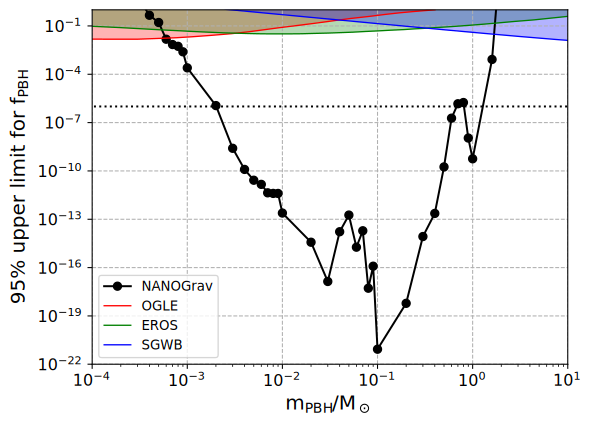
\includegraphics[width=0.8\textwidth]{fpbh_upper.pdf}
    \bicaption[从NANOGrav 11年数据集中得到的原初黑洞占冷暗物质丰度$\fpbh$的$95\%$上限关于原初黑洞质量$m_{\rm{PBH}}$的函数。图中还显示了来自OGLE微透镜(OGLE)、EROS/MACHO微透镜(EROS)和随机引力波背景的结果。水平虚线对应的是$10^{-6}$。]{\label{fpbh_upper} 从NANOGrav 11年数据集中得到的原初黑洞占冷暗物质丰度$\fpbh$的$95\%$上限关于原初黑洞质量$m_{\rm{PBH}}$的函数。图中还显示了来自OGLE微透镜(OGLE)\cite{Niikura:2019kqi}、EROS/MACHO微透镜(EROS)\cite{Tisserand:2006zx}和随机引力波背景\cite{Chen:2019irf}的结果。水平虚线对应的是$10^{-6}$。}{The $95\%$ upper limits on the abundance of primordial black holes
        in cold dark matter $\fpbh$ as a function of the primordial black hole mass $m_{\rm{PBH}}$ from the
        NANOGrav 11-year data set. 
        Results from OGLE microlensing (OGLE) \cite{Niikura:2019kqi},
        EROS/MACHO microlensing (EROS) \cite{Tisserand:2006zx}, 
        and SGWB \cite{Chen:2019irf} are also shown. 
        The horizontal dotted line corresponds to $10^{-6}$.}
\end{figure}

\Fig{A_upper}给出了从NANOGrav 11年数据集得到的功率谱振幅$A$的$95\%$置信上限和贝叶斯因子作为峰值频率$\fstar$的关系。尽管贝叶斯因子分布中有两个峰值,但两个峰值值都小于$3$,这意味着数据中信号的存在是``不值一提"的 \cite{BF}。由于每个峰值频率的贝叶斯系数$B_{10}$小于$3$,说明数据中与只含有噪声是一致的。\Fig{fpbh_upper}给出了原初黑洞在暗物质中的丰度$\fpbh$的$95\%$的置信度上限作为原初黑洞质量$m_{\rm{PBH}}$的关系。\Eq{mkrelation}给出了$m_{\rm{PBH}}$与$\fstar$的关系,而\Eq{fpbh}给出了$\fpbh$与$A$的关系。我们的结果意味着当前的PTA数据集已经能够通过标量诱导引力波对原初黑洞的丰度进行严格的限制。由\Fig{fpbh_upper}可知,在$[2\times 10^{-3}, 7\times 10^{-1}] \Msun$的质量范围内,原初黑洞的丰度小于$10^{-6}$。


我们首次在NANOGrav 11年数据集中搜索伴随着原初黑洞形成而不可避免产生的标量诱导力波的信号。由于没有发现显著的信号,我们对峰值频率范围$[1.5\times 10^{-9}, 3\times 10^{-6}]$Hz和质量范围$[4\times10^{-4}, 1.7]\Msun$的原初黑洞的丰度给出了$95\%$的上限。特别是,原初黑洞在$[2 \times 10^{-3}, 7\times 10^{-1}] M_\odot$ 质量范围内的丰度小于$10^{-6}$,这比已有文献中对这个质量范围的观测限制都要好得多。虽然我们假设原初黑洞的质量函数是单色的,但由于即使对于具有扩展质量分布的情况,标量诱导引力波的振幅也大致由标量功率谱的峰值振幅决定,因此,从NANOGrav 11-yr数据中应该可以获得类似的标量功率谱峰值振幅约束。因此,也可以预期具有扩展质量分布的原初黑洞的丰度也会受到严格的限制。原则上,对具有扩展质量分布的情况的精确分析是模型模型依赖的。我们将在未来考虑原初黑洞有质量分布的情况。

%The constraint covers a wide 原初黑洞 mass window from $10^{-4}M_{\odot}$ to solar-mass window. At the most frequency band, corresponding to the subsolar-mass window $\sim0.1M_\odot$, the upper limit reach $\sim10^{-38}$. 

%Also, it is as expected that bringing the third-order correction into consideration leads to a several orders of magnitude difference $f_{\rm{pbh}}$. This is because $f_{\rm{pbh}}$ is very sensitive to $A$. It can be estimated from Eq.~(\ref{beta}) that
%\e
%\Delta f_{\rm{pbh}}= \frac{\zeta_c(\zeta_c-3A)}{6\sqrt{6\pi}A^{3}}\exp\(-{\zeta_c\over 2A}\)\Delta A.
%\q
%The third-order correction would lead to about a $10\%$ increase of the amplitude $\Delta A\approx0.1$. For a typical value $A=0.01$, the relative correction of the abundance would be $\Delta f_{\rm{pbh}}/f_{\rm{pbh}}\approx500$, rendering the higer-order corrections of the 标量诱导引力波 are indispensable.



%\begin{figure}[htbp!]
%\centering
%\includegraphics[width=0.8\textwidth]{A_post.pdf}
%\bicaption{当峰值频率为$\fstar=\rm{yr}^{-1}$时,曲率扰动幅度$A$的后验分布。 
%}{The posterior distribution of curvature perturbation
%amplitude $A$ when peak frequency $\fstar=\rm{yr}^{-1}$.}
%\label{A_post} 
%\end{figure}
%
%\begin{figure}
%\subfloat{\includegraphics[width=0.45\textwidth]{J0613-0200.pdf}}\hspace{5mm} 
%\subfloat{\includegraphics[width=0.45\textwidth]{J1012+5307.pdf}}\\
%\subfloat{\includegraphics[width=0.45\textwidth]{J1600-3053.pdf}}\hspace{5mm} 
%\subfloat{\includegraphics[width=0.45\textwidth]{J1713+0747.pdf}}\\
%\subfloat{\includegraphics[width=0.45\textwidth]{J1744-1134.pdf}}\hspace{5mm} 
%\subfloat{\includegraphics[width=0.45\textwidth]{J1909-3744.pdf}}
%\bicaption{当峰值频率$\fstar=\rm{yr}^{-1}$时,我们分析中使用的6颗脉冲星(见\Table{pulsars})的红噪声振幅$\ARN$和光谱指数$\gRN$的一维和二维边际化后验分布。每个子图给出了在$68\%$和$95\%$的置信度等值线。
%}{The one- and two-dimensional marginalized posterior distributions of the red-noise amplitude $\ARN$ and spectral index $\gRN$ for the $6$ pulsars
%(see \Table{pulsars}) used in our analysis when peak frequency
%$\fstar=\rm{yr}^{-1}$. 
%For each sub-figure, the contours are at $68\%$ and $95\%$ confidence levels
%respectively. }
%\label{psrs_post}
%\end{figure}

%However, the constraint given by this paper strongly depends on the assumption that the comoving curvature perturbations obey Gaussian statistics. This is because 原初黑洞 are supposed to form from the tail of the probability density function, so that the possibility to form a 原初黑洞 is extremely sensitive to non-Gaussianity \cite{Young:2018lec}. It has been studied in \cite{Cai:2018dig,Cai:2019amo,Cai:2019elf} that non-Gaussianity may intensely suppress the amplitude of the 标量诱导引力波 so that the null detection of 标量诱导引力波 may be given rise to large primordial non-Gaussianity.